\indent Para estudiar el funcionamiento de nuestro algoritmo frente a la problematica planteada, elaboramos diversos tests que ser\'an enunciados a continuaci\'on.\\

\begin{center}
 \subsubsection*{Familia 1: Sin Soluci\'on 1. La capacidad de la mochila no es apta para ganar ciertos gimnasios}
\end{center}

Para que no haya soluci \'on asignamos la capacidad de la mochila inferior a la cantidad de pociones necesarias para ganar en algun gimnasio.\\
 
\vspace*{0.3cm} \vspace*{0.3cm}
  \begin{center}
 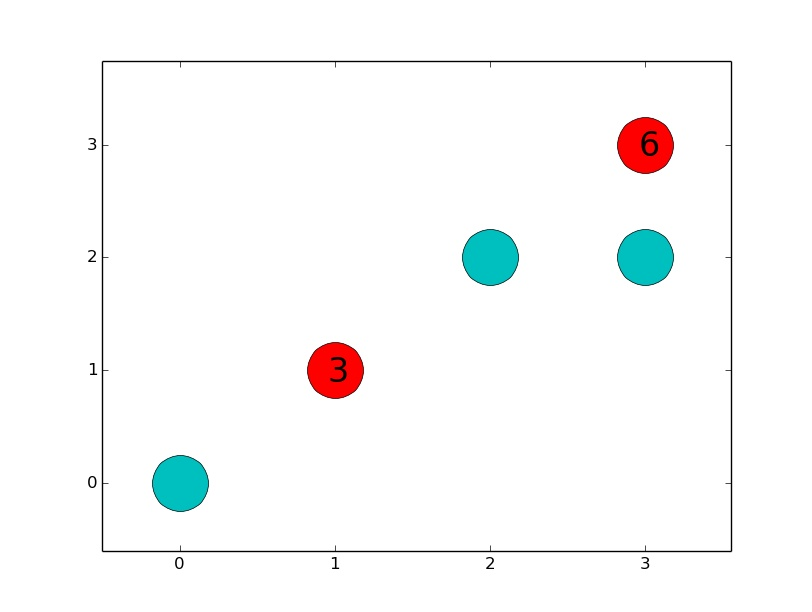
\includegraphics[scale=0.60]{./EJ1/sinSolucion.jpeg}
\\{$Ejemplo$ \ 1.1 - $Caso$ $Sin$ $Soluci$\'on}
  \end{center}
  \vspace*{0.3cm}

---> HABRIA Q AGREGAR EL GRAFO DEL PYTHON O MODIFICAR LAS POSICIONES EN ESTE\\

\begin{center}
 \subsubsection*{Familia 2: Sin Soluci\'on 2. La cantidad de pokeparadas no es suficiente para ganar todos los gimnasios}
\end{center}

Para que no haya soluci \'on asignamos una cantidad menor de pokeparadas necesarias a la suma total de pociones necesarias para poder vencer en todos los gimnasios\\
 
\vspace*{0.3cm} \vspace*{0.3cm}
  \begin{center}
 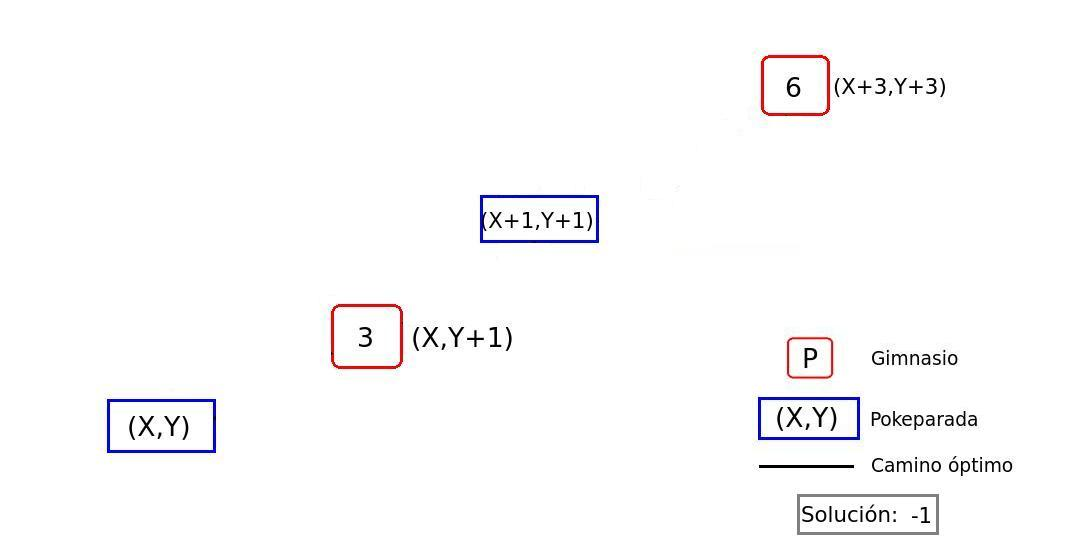
\includegraphics[scale=0.6]{./EJ1/sinSolucion1.jpeg}
 \\{$Ejemplo$ \ 1.2 - $Caso$ $Sin$ $Soluci$\'on}
  \end{center}
  \vspace*{0.3cm}
  
\begin{center}
 \subsubsection*{Familia 3: Ning\'un gimnasio necesita pociones para ser vencido}
\end{center}

En este caso, como el titulo lo indica, no hay gimnasio que necesite pociones para ser vencido, todos tendran valor 0.
 
\vspace*{0.3cm} \vspace*{0.3cm}
  \begin{center}
 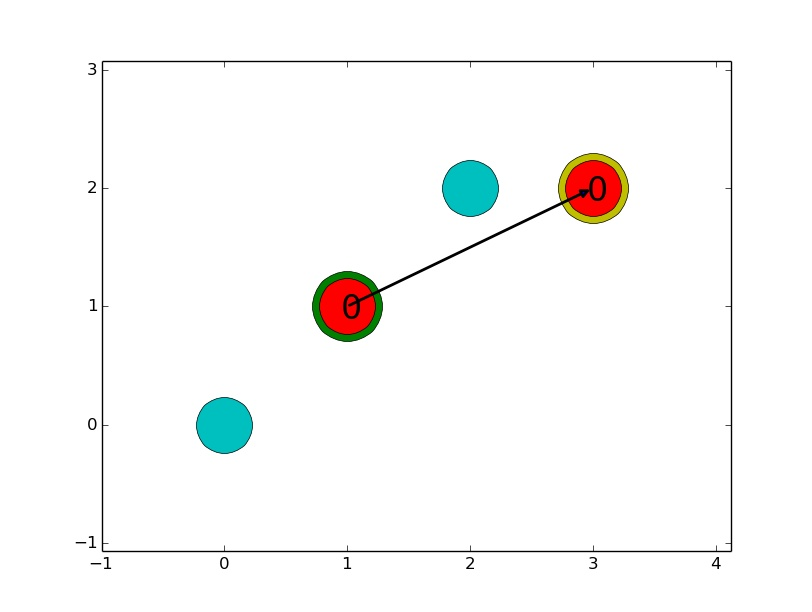
\includegraphics[scale=0.6]{./EJ1/gym0.jpeg}
\\ {$Ejemplo$ \ 1.3 - $Caso$ $Todos$ $Los$ $Gym$ $Con$ $0$}
  \end{center}
  \vspace*{0.3cm}

\begin{center}
  \subsubsection*{Familia 4: Alg\'un gimnasio necesita pociones para ser vencido}
\end{center}

A diferencia de la familia anterior, en este caso solo algunos gimnasios no necesitan pociones para ser vencidos.\\

------>> FALTA HACER
\vspace*{0.3cm} \vspace*{0.3cm}
  \begin{center}
 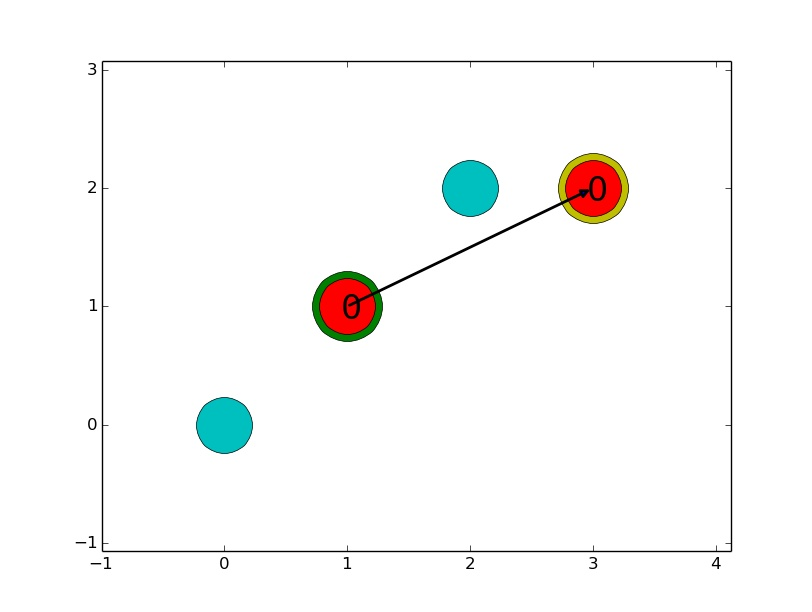
\includegraphics[scale=0.6]{./EJ1/gym0.jpeg}
\\ {$Ejemplo$ \ 1.4 - \textit{Algunos gimnasios con 0}}
  \end{center}
  \vspace*{0.3cm}
------>> FALTA HACER\\

\begin{center}
  \subsubsection*{Familia 5: Se reciben pokeparadas y gimnasios en orden}
\end{center}

Este caso se da cuando se reciben las pokeparadas y gimnasios con el camino minimo ya armado.

\vspace*{0.3cm} \vspace*{0.3cm}
  \begin{center}
 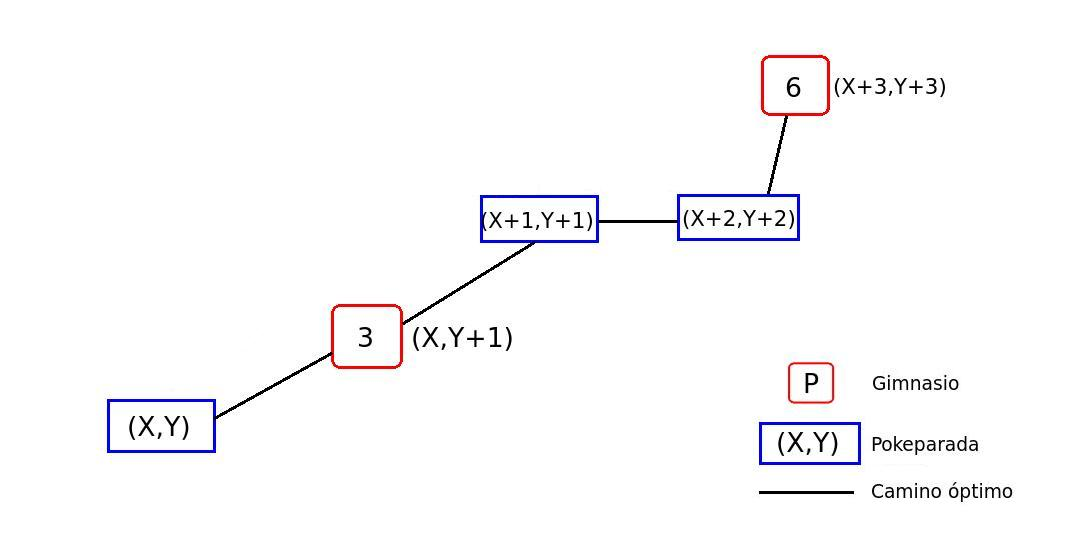
\includegraphics[scale=0.6]{./EJ1/optima.jpeg}
\\ {$Ejemplo$ \ 1.5 - \textit{Camino minimo recibido como entrada}}
  \end{center}
  \vspace*{0.3cm}

\begin{center}
  \subsubsection*{Familia 6: Entrada fuera de orden (orden diferente para lograr el óptimo)}
\end{center}

Este estilo de familia presenta a los gimnasios y pokeparadas desordenados en referencia a las posiciones, es decir, para ganar a cierto gimnasio es necesario pasar por una cantidad puntual de pokeparadas las cuales estan de un lado y del otro de dicho gimnasio.
---->Explicar bien este

\vspace*{0.3cm} \vspace*{0.3cm}
  \begin{center}
 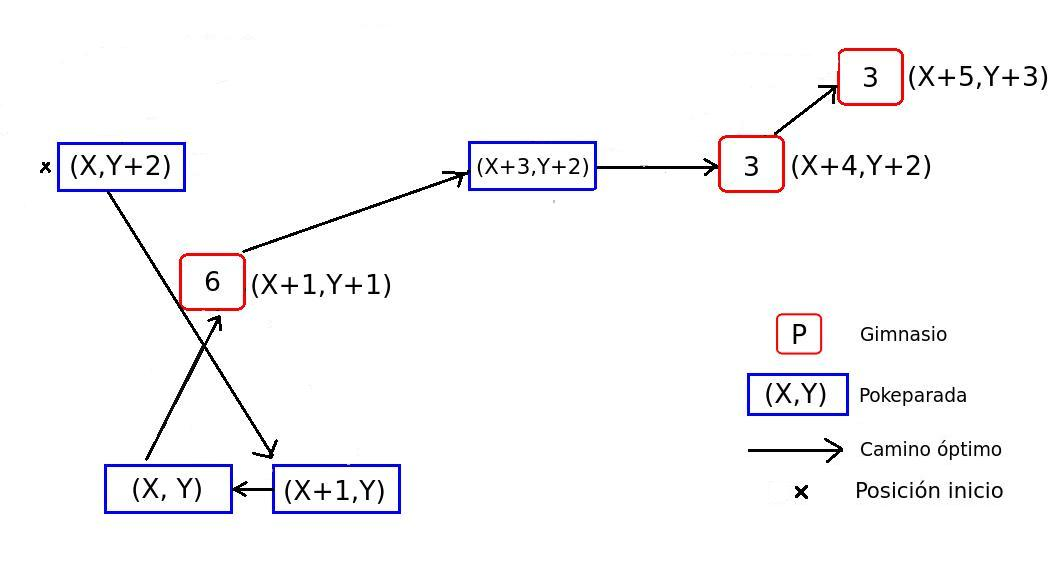
\includegraphics[scale=0.6]{./EJ1/desorden.jpeg}
\\ {$Ejemplo$ \ 1.6 - \textit{Camino desordenado}}
  \end{center}
  \vspace*{0.3cm}

\begin{center}
  \subsubsection*{Familia 7: Anillos de pokeparadas y gimnasios}
\end{center}

Este estilo de familia se elabora de la forma en la cual se tengan todos los gimnasios en ciertas posiciones, donde el conjunto total de estos nos devuelva una forma de anillo, mientras que las pokeparadas presenten la misma forma que los gimnasios a una distancia euclidea id\'entica entre pokeparada-gimnasio.\\

--->HACER EL GRAFICO PARA ESTE
\vspace*{0.3cm} \vspace*{0.3cm}
  \begin{center}
 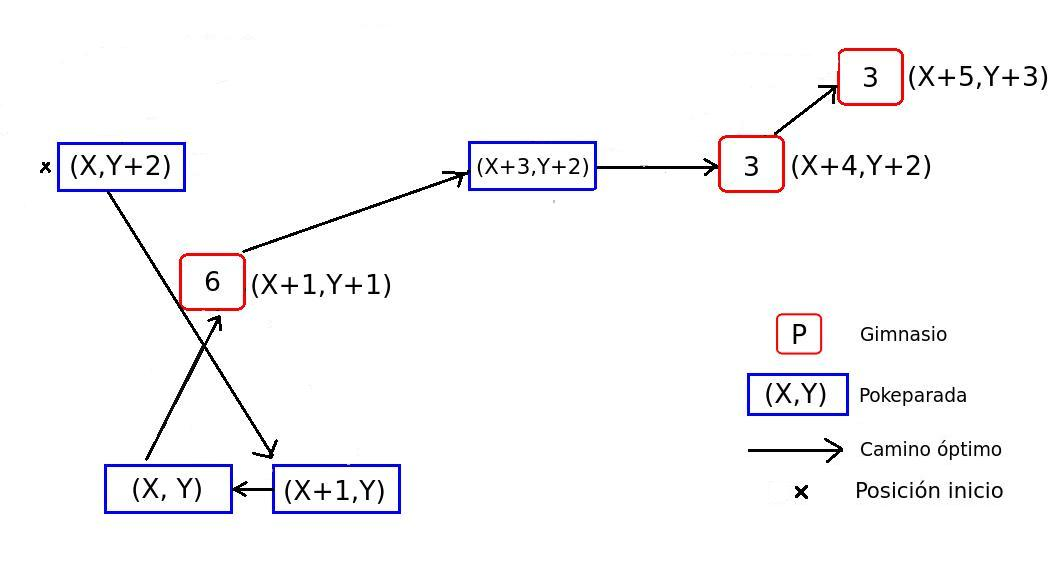
\includegraphics[scale=0.6]{./EJ1/desorden.jpeg}
\\ {$Ejemplo$ \ 1.6 - \textit{Camino desordenado}}
  \end{center}
  \vspace*{0.3cm}
--->HACER EL GRAFICO PARA ESTE\\


\indent Luego de haber enunciado cada familia de test, veremos que es lo que sucede al ir variando los parámetros de entrada para cada familia, de manera tal que, a medida que N y M crecen linealmente podamos observar que sucede con cada familia de casos (es decir, las familias se mantienen, solo varia el tamaño de la entrada en todos los casos).\\
Se comienza, por lo tanto, con una entrada de un gimnasio y un pokeparada y se la aumenta en cada test en uno hasta llegar a un total de 20 elementos entre ambos conjuntos (Debido al poder de computo, no es posible trabajar con instancias de mayor tamaño). De manera que no hay desigualdades y todas las familias se miden en instancias de igual tamaño.\\

Para obtener dichas instancias se realizaron aproximadamente unas 20 corridas con el mismo input y se tom\'o el promedio de las mismas en cada instancia para obtener un valor m\'as cercano a la media.\\ 

Se puede observar en el  gráfico 1.1, siete funciones, que representan el tiempo de ejecuci\'on de las familias de casos mencionadas en el apartado anterior:\\

\begin{enumerate}
\item Sin Solucion 1. La capacidad de la mochila no es apta para ganar ciertos gimnasios
\item Sin Solucion 2. La cantidad de pokeparadas no es suficiente para ganar todos los gimnasios
\item Ning\'un gimnasio necesita pociones para ser vencido
\item Alg\'un gimnasio necesita pociones para ser vencido
\item Se reciben pokeparadas y gimnasios en orden
\item Entrada fuera de orden (orden diferente para lograr el óptimo)
\item Anillos de pokeparadas y gimnasios
\end{enumerate}


----->> FALTAN TERMINAR LAS MEDICIONES PARA HACERLO Y HACER EL TEST DEL ANILLO\\
\vspace*{0.3cm} \vspace*{0.3cm}
  \begin{center}
% 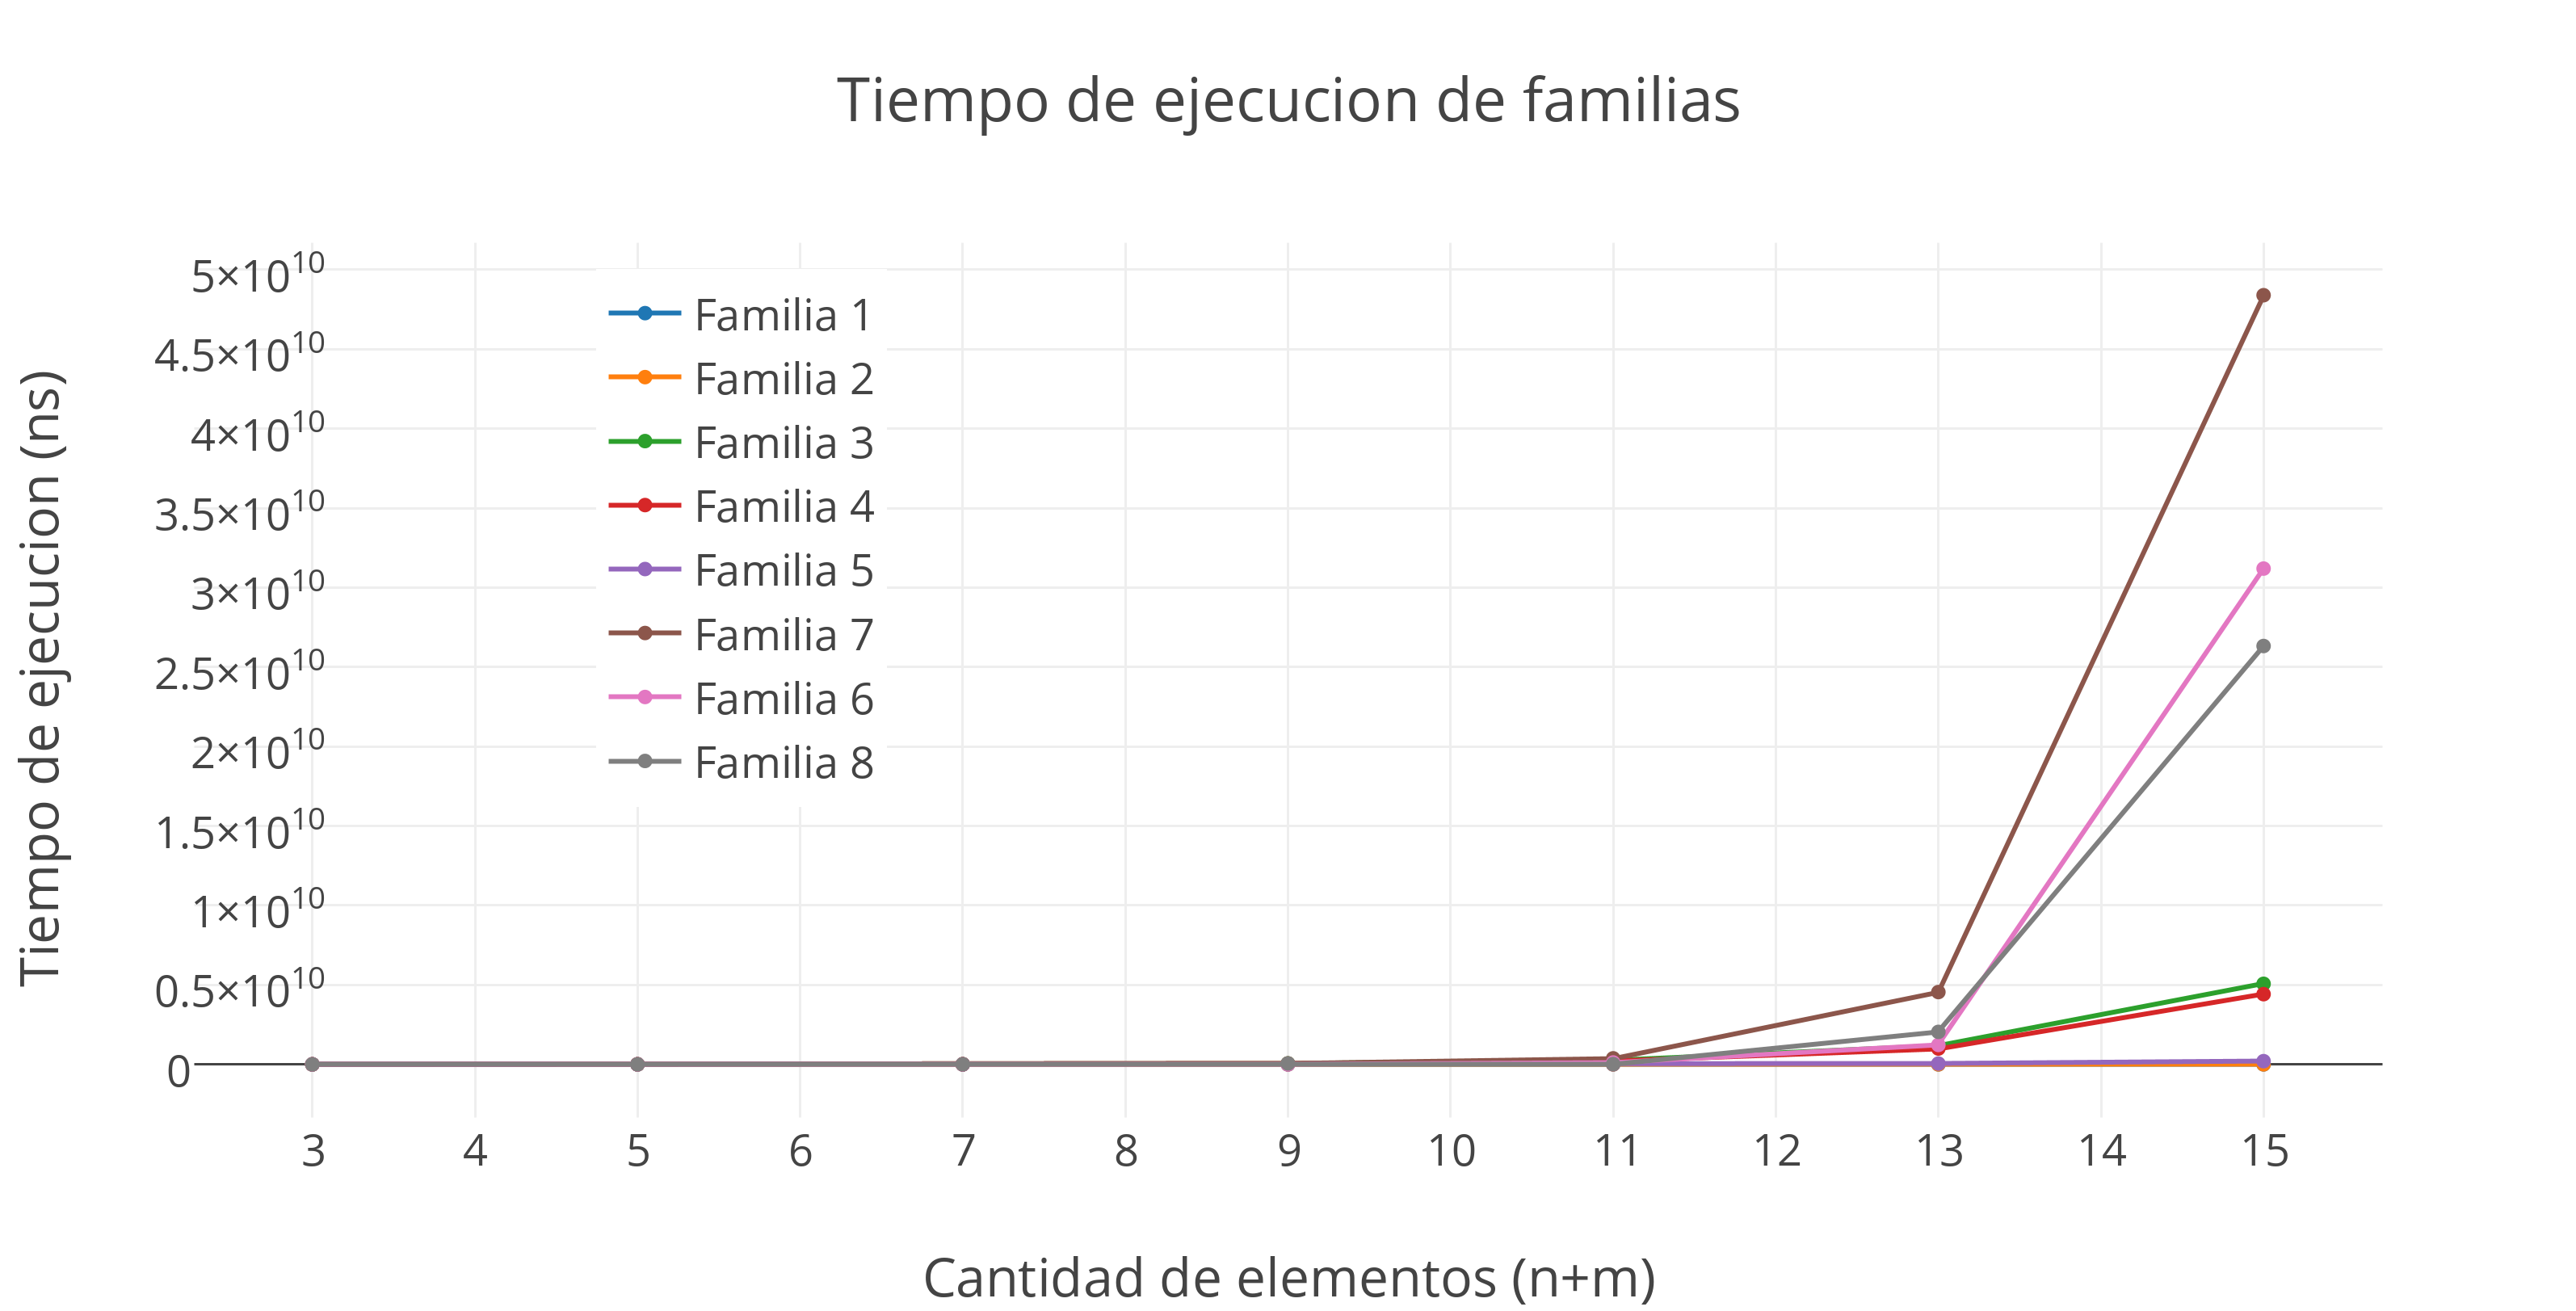
\includegraphics[scale=0.5]{./EJ1/comparativo.png}
 {Gr\'afico \ 1.1 - $Comparativo$}
  \end{center}
  \vspace*{0.3cm}
  
Se puede notar que la familia 1 "\textbf{La capacidad de la mochila no es apta para ganar ciertos gimnasios}" y la n\'umero 2 "\textbf{La cantidad de pokeparadas no es suficiente para ganar todos los gimnasios}", presentan una mejor performance en relaci\'on a las otras. Esto se debe a que se realizan dos podas para chequear si la entrada posee o no soluci\'on. Puntualmente, la familia uno es un poco mejor a la segunda debido a que en la implementaci\'on de dicha poda a penas chequea que existe al menos un gimnasio con mayor cantidad de pociones para ser vencido que la capacidad corta directamente la ejecuci\'on y finaliza, mientras que para la segunda, la poda implementada debe chequear gimnasio por gimnasio la cantidad de pociones necesarias para sumarlas y luego chequear si la cantidad de pokeparadas alcanzar\'an para poder vencer en todos los gimnasios.\\

----->VER SI HACEMOS UN GRAFICO CON LAS DOS FAMILIAS \\

Uno de los peores casos para nuestro algoritmo es la familia 7 "\textbf{Anillos de pokeparadas y gimnasios}", que sucede cuando por ejemplo, todos los caminos tienen igual longitud. Esto se da as\'i ya que nuestro algoritmo chequea todas las ramas posibles del backtraking y como todos pueden ser soluci\'on posible avanza por todos llegando al final de cada rama con el mismo valor en todos los posibles caminos.\\

-----> HACER EL GRAFICO DE ANILLOS\\

Veamos en detalle como se comportan el mejor y peor caso con respecto a la complejidad calculada.\\

  \vspace*{0.3cm} \vspace*{0.3cm}
  \begin{center}
%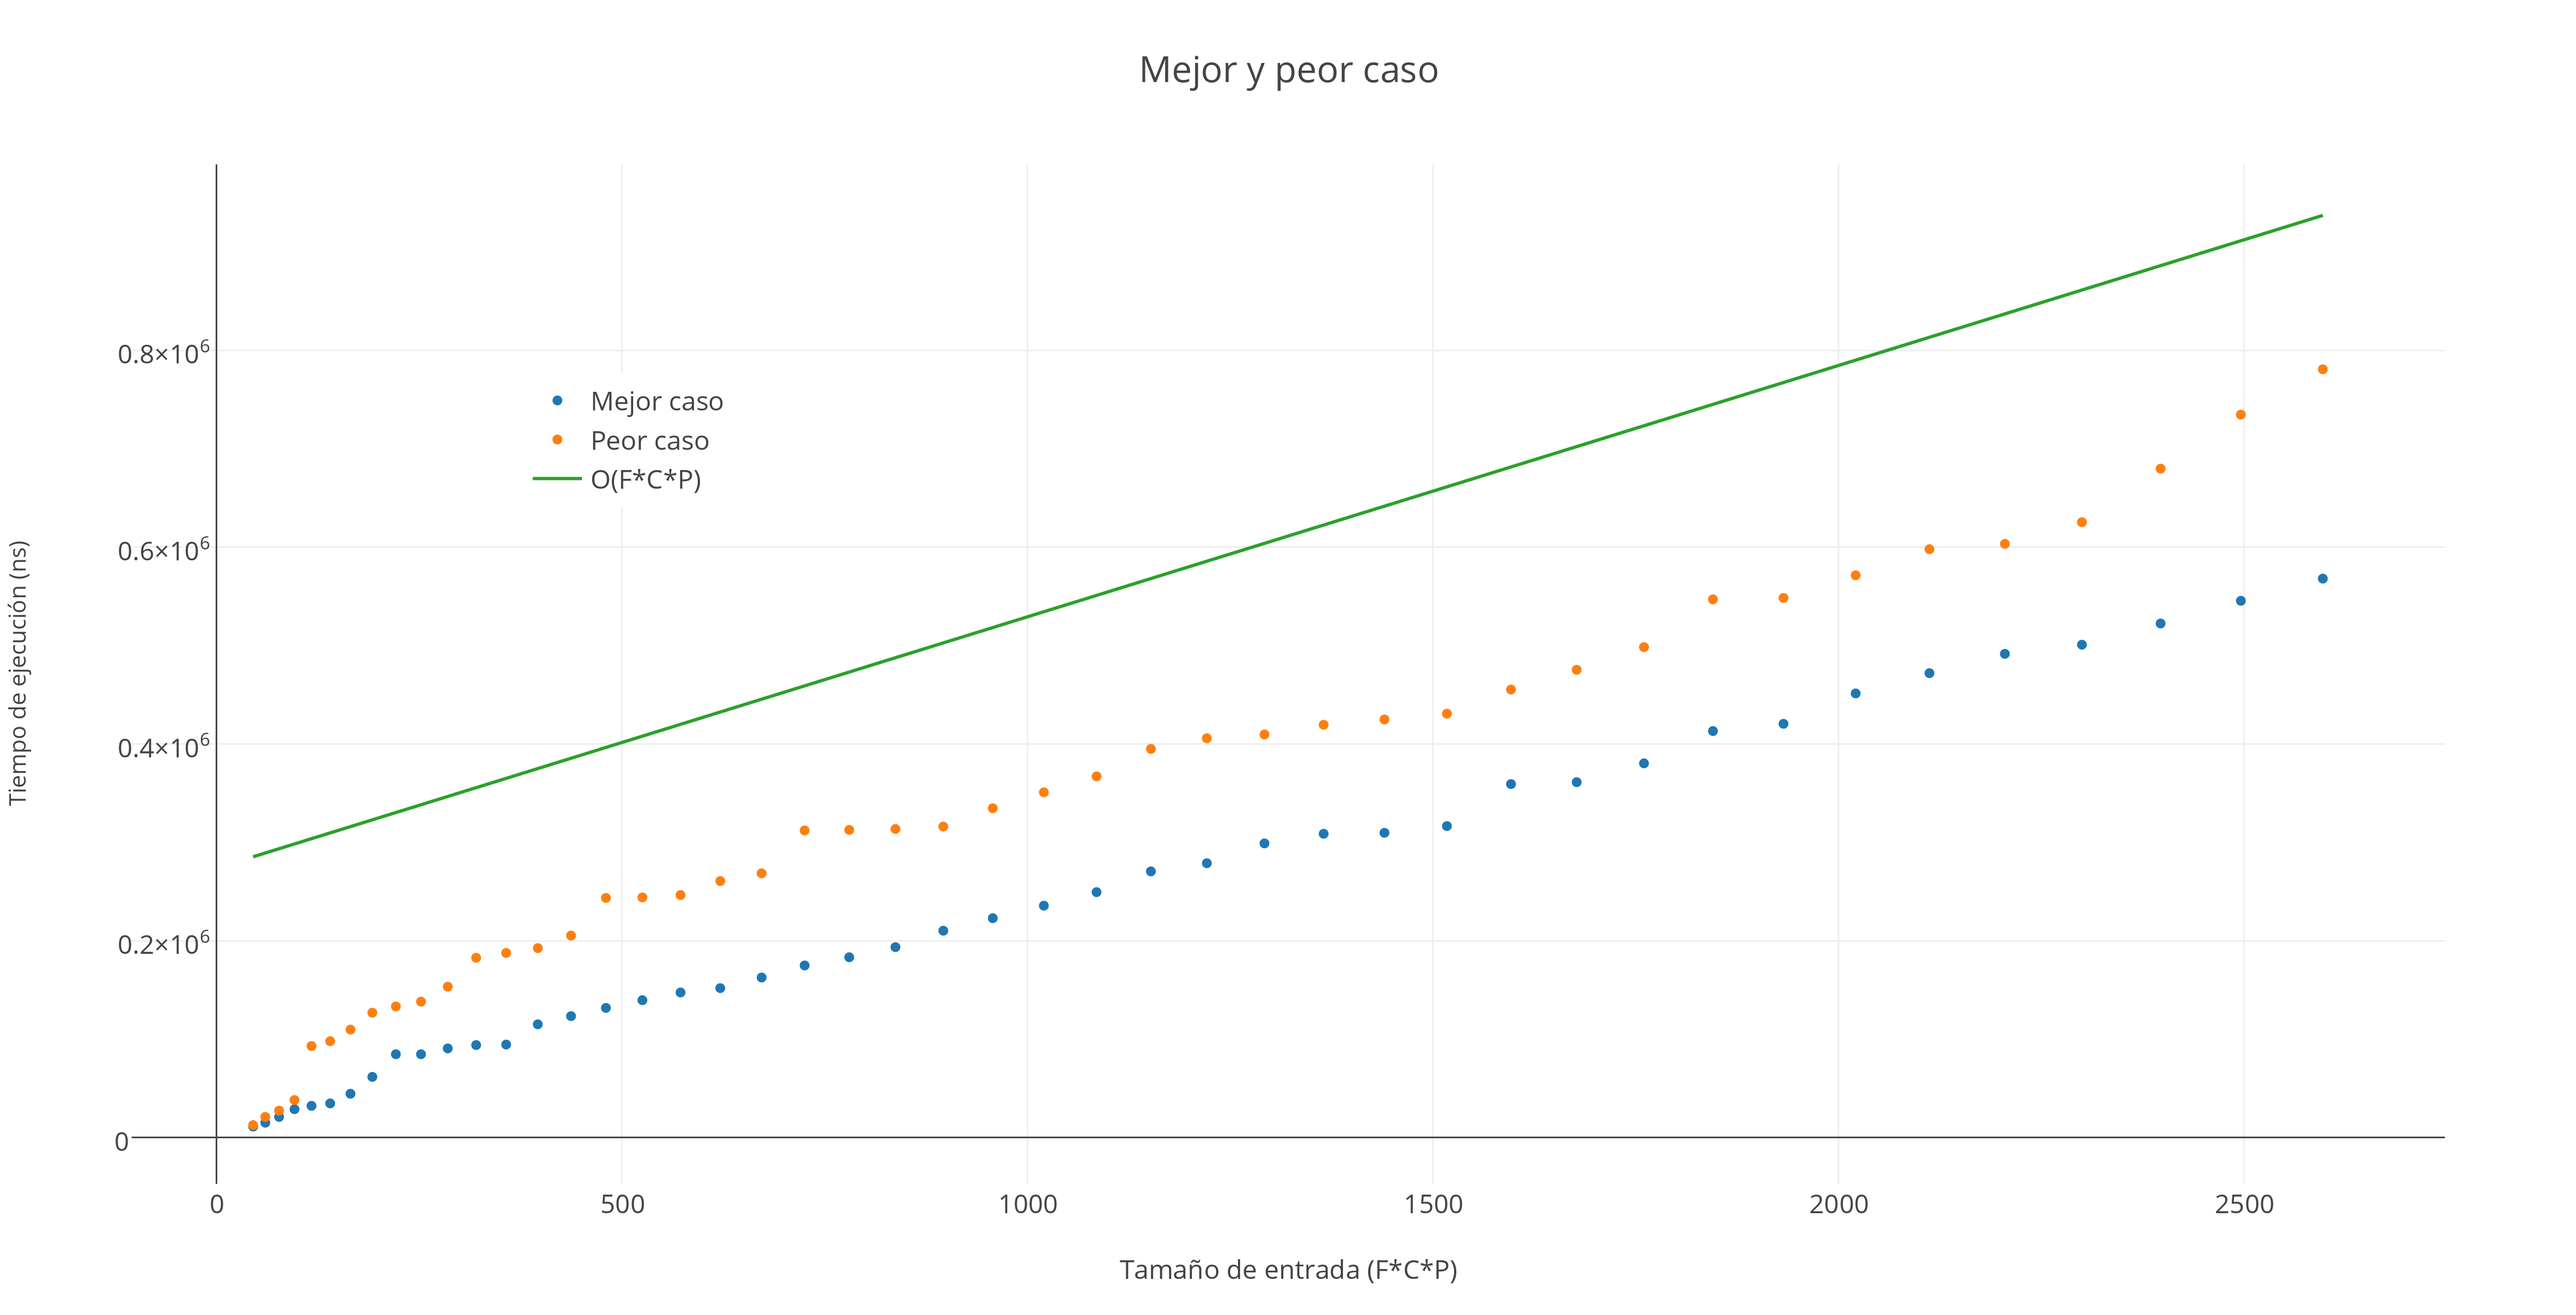
\includegraphics[scale=0.5]{./EJ1/MejorYPeorCaso.png}
{Gr\'afico 1.5 - $Comparativo$}
  \end{center}
  \vspace*{0.3cm}

Podemos ver en este gr\'afico comparativo como las familias est\'an acotadas por la funci\'on de la complejidad te\'orica calculada.\\

